%
% File naaclhlt2018.tex
%
%% Based on the style files for NAACL-HLT 2018, which were
%% Based on the style files for ACL-2015, with some improvements
%%  taken from the NAACL-2016 style
%% Based on the style files for ACL-2014, which were, in turn,
%% based on ACL-2013, ACL-2012, ACL-2011, ACL-2010, ACL-IJCNLP-2009,
%% EACL-2009, IJCNLP-2008...
%% Based on the style files for EACL 2006 by 
%%e.agirre@ehu.es or Sergi.Balari@uab.es
%% and that of ACL 08 by Joakim Nivre and Noah Smith

\documentclass[11pt,a4paper]{article}
\usepackage[hyperref]{naaclhlt2018}
\usepackage{times}
\usepackage{latexsym}

\usepackage{url}
\usepackage{graphicx} %package to manage images
\graphicspath{ {/} }

\aclfinalcopy % Uncomment this line for the final submission
%\def\aclpaperid{***} %  Enter the acl Paper ID here

\setlength\titlebox{3cm}
% You can expand the titlebox if you need extra space
% to show all the authors. Please do not make the titlebox
% smaller than 5cm (the original size); we will check this
% in the camera-ready version and ask you to change it back.

\newcommand\BibTeX{B{\sc ib}\TeX}

\title{A Scalable Augmentation of the Student Education Process}
\author{Anonymous MAIS Submission
}
\date{}

% \author{Bhairav Mehta \\
%   University of Michigan \\
%   {\tt bhairavm@umich.edu}
%   \And
%   Adithya Ramanathan \\
%   University of Michigan \\
%   {\tt adithram@umich.edu}}
% \date{}

\begin{document}
\maketitle
\begin{abstract}
  We present a novel intelligent tutoring system, which builds upon well-established hypotheses in educational psychology and encompasses them inside of a scalable software architecture. Specifically, we incorporate the benefits of knowledge vocalization \cite{TODO}, parallel learning \cite{TODO}, and immediate feedback \cite{TODO} in the context of student learning. Driven by free, online resources, our work scales easily in terms of class size while still operating at the granularity of individual students. Additionally, we allow teachers to retain full control of the outputs, and provide student statistics to help them better steer their classroom discussions. Our experiments show promising results, and cement our hypothesis that the system is flexible enough to serve a wide variety of purposes in a classroom setting.
\end{abstract}
\section{Introduction}
One notable constant throughout entire human eras has been education. Despite changing mediums, from paper to pixels, the \textit{structure} of education has stayed nearly identical: sequential, isolated learning, bookended by exams and benchmarked by grades. Many technological solutions proposed don't make good use of either the educational infrastructure already in place, or the expertise of teachers who are interacting with the technology day-to-day. 

In this paper, we develop a novel framework that can replicate some factors cited by educational psychologists that are conducive to learning; specifically, when students vocalize what they've learned, get feedback on those responses, and learn about related topics when they are stuck on the main one, knowledge retention has been proven to increase \cite{TODO}. We ask students to vocally answer questions created by their teacher, who provided pertinent data sources when creating the question. We then perform semantic similarity tests between a student answer and the key concepts extracted from source data, and provide feedback to student about their performance and bring them to other questions that will help cover their gaps in knowledge. We stay true to the unofficial education-technology motto of minimizing teacher investment while maximizing student impact \cite{norris_soloway02/12/18}, and develop a pipeline that uses state-of-the-art methods in machine learning to augment the education process.
\subsection{Related Work}
Education technology (ET) is defined as the "practice of facilitating learning and improving performance by creating, using, and managing appropriate technological processes" \cite{hlynka_jacobsen}. Some of the best ET applications on the market offer flexibility by allowing the educator to determine their importance in the classroom. The apps constantly interact with the student in multiple ways, and offer ease of setup through pre-built curricula. Yet, many of these same apps are still constrained by the fact that their materials are entirely expert-curated. Our approach builds on the principles of interaction and feedback, but goes further by providing a way to intelligently build curricula and provide recommendations to struggling students by using only a few, teacher-provided links or text sources.
\section{Implementation}
\subsection{Pre-Teacher Setup} \label{pre_teacher}
% Turn Datasets + Raw Text + GMB = 2 sentences
For each subject area supported by our framework, we create a tf-idf index \cite{Ramos_usingtf-idf} using a hand-crafted list of seed URLs that we believe are pertinent to the topic (i.e the subject of US History may have Wikilinks to different eras in American History). We use standard text preprocessing techniques \cite{TODO} in the creation of these indices, and separating them by subject allows us to mitigate the issue of domain transfer \cite{TODO} with tf-idf indices.
\subsection{Teacher Usage}\label{teacher}
Upon creating a class, the teacher selects a subject area that roughly corresponds to the class being taught, in order to match a relevant tf-idf index to the class. The teacher, then posed to create questions, is asked to provide two pieces of information: a Question Title (seen by the student when asked to answer), and Data Sources. The data sources, links or blocks of text, are assumed to be relevant to the question, and are then preprocessed using the same standard techniques as in Section \ref{pre_teacher}. Once we have cleaned text, we use a LSTM-CRF model \cite{TODO}, trained on the Annotated Groningen Meaning Base \cite{TODO}, to extract named entities (NE). In parallel, we run the text through TextRank \cite{TODO} \cite{TODO Barrios}, and retrieve a list of key concepts (KC) from the source. We calculate the score for each word using a weighted score of it's tf-idf weight, and indicator functions corresponding to its presence in either the NE or KC lists.
\begin{equation}
    s(w) = TF(w) + \alpha \I[KC(w)] + \beta \I[NE(w)]
\end{equation}
where $TF(w)$ is the tf-idf score of the word, and $\alpha$ and $\beta$ are empirically-set hyperparameters. If appropriate, we combine the words into phrases using the two lists of NEs and KCs, as well as the NLTK Multiword Expression Tokenizer \cite{TODO}, and assign the phrase the sum of its component scores. We return to the teacher a list of (concept, score) pairs. The teacher can then manually adjust any phrases and their corresponding score values, and can enable visibility for students.
\subsection{Student Usage}
\subsubsection{Answering}
When a student enrolls in a class, he will see the questions proposed by the teacher, only with the question title. As the teacher picked data sources presumably related to class material, the student will be able to enable his microphone, and start answering the question by speaking to the computer using knowledge from class or homework. To handle speech-to-text, we utilize DeepSpeech \cite{TODO}, and with the transcripted text, we preprocess it with the same methods used in Section \ref{pre_teacher}. From there, we tokenize the answer, and then score the answer by checking for token existence in the list of phrases associated with the question. We contribute the phrase's full score even for partial hits, although more sophisticated methods could be used.
\subsubsection{Recommendations}
With the score and a visual representation of which of the words in his answer matched up with key concepts associated with the question, we provide recommendations to other questions. 
% Figure Here!

\section{Results}

\section{Conclusion}
% \subsection{System}
% \subsubsection{Raw Text Extraction}
% Using the raw text harvested from the spider described in Section \ref{data_raw_text}, we remove stopwords, and stem the remaining text using the NLTK Wordnet Lemmatizer \cite{Fellbaum1998}. With this preprocessed text, we concatenate all of the web pages to generate a tf-idf index \cite{Ramos_usingtf-idf}. As we assume that our text samples are representative of the true distribution of words, our tf-idf index serves as a proxy of how important and rare particular words are to the whole of the corpus. Through experimentation testing the ability of these indices to transfer across domains (i.e having been generated on a list of seed URLs from American History, how accurately could we gauge the importance of words from Psychology text), we find that these indices are also subject to the domain transfer issue discussed in the Related Work. To mitigate this issue, we envision a tf-idf index being generated per subject (i.e History, Psychology, etc).

% \subsubsection{Named Entity Recognition}
% The Named Entity module is utilized in two phases. First, there is a training phase where the model is trained to predict named entities in raw text using the Annotated Groningen Meaning Base as a training corpus. Secondly, there is a classification phase where the trained model is stored into a pickle file, and utilized to predict named entities from raw text. 

% Training begins with preprocessing and feature engineering of the training corpus. The corpus is preprocessed into sentence tuples. The entire training corpus is reconstructed as a list of tuples, where each sentence is broken down into tuples of word, part-of-speech, and it’s respective named entity tag. Given this reformatted training corpus, the data is converted into features extracting certain key identifiers for each word in a sentence such as case, position, part-of-speech, contextual part-of-speech, whether the word is a number, and whether the word is a title. Additionally, the features are engineered to consider both the previous and next word, and their respective values as features as well.  At this point, the system has reformatted the Annotated Groningen Meaning Base into a collection of feature vectors. 

% For our use case, we utilize a Conditional Random Fields model. The CRF model performs a class of statistical modeling focused on conditional probability modeling. Additionally, CRF models fall into the class of sequential models, and is thus effective in this use case by considering neighboring terms and context when making conditional probability based predictions. The model is trained using the feature vectors previously constructed. The feature map appears as follows:

% $$\phi(x_1, ...,x_m, s_1,...,s_m)$$ where $x \in$ feature vectors and $s \in $ named entity labels.

% The feature vectors are processed and considered using a log likelihood function:
% $$L(w) = \sum_{i=1}^{n}log(p(s^i|x^i; w) - \frac{\lambda_2}{2} ||w||^2_2 - \lambda_1||w||_1$$

% Where the conditional probability function is modeled as:
% $$p(s|x;w) = \frac{exp(w \cdot \phi(x,s))}{\sum_{s'}exp(w \cdot \phi(x,s'))}$$

% And the parameter vector, where the two parameter terms (which helps alleviate complexity) are:
% $$\frac{\lambda_2}{2} ||w||^2_2$$ $$\lambda_1||w||_1$$

% The parameter vector is estimated as:
% $$w^* = \arg\max_{w\in \mathbb{R}^d}L(w)$$

% Based on training, and cross validation tests, we chose to modify the L1 Hyperparameter by increasing the value. This helped the model further focus on context rather than pure memorization and led to better empirical results. Once the model has been trained, we dump the model into a pickle file. The pickle file serves as a saved, binary export of the model such that we can later access the model to make predictions rather than retraining the model at each occurrence. 

% The second phase begins by taking in raw text as input. This raw text is then split into sentences, and each sentence is then further broken down into tuples. Using the NLTK (Natural Language Toolkit) library, the part-of-speech tagger is utilized to breakdown the sentence into tuples of term, and part of speech. At this point, we convert these reformatted sentences into feature vectors, in the exact same manner as the training data. We then make predictions regarding each term.If the parameter vector is estimated, the most likely tag for a label can be found using.
% $$s^* = argmax_{s}p(s|x;w^*)$$

% At this point, we parse out all terms that are not considered named entities, and soley keep those original terms that are considered to be named entities. 
% \subsubsection{Topic Scoring and Ranking}

% Now, given a trained NER system and a tf-idf index that will serve as a proxy for importance, we can start to evaluate our system. During deployment, we envision that this is the first step an actual teacher would be involved. 

% The system prompts the user for a question title (which will be shown to the student), and then asks the user to provide source documents that the expert user deems to be relevant to the question posed. The source documents can be raw text, or URLs which are preprocessed the same way as described in Section  \ref{data_raw_text}. From there, we run each processed word through a scoring module

% $$score_q(w) = tfidf(w) + a*SI(w) + b*NE(w)$$

% where $SI(w)$, short for semantic importance, is a multiplier if the particular word was in a section heading in the original HTML and a constant if from raw text, $NE(w)$ is a multiplier if the word is present in any of the named entities extracted from the text using the NER model, and $a$ and $b$ are empirically defined hyperparameters. If the word comes from raw text inputted by the user, $SI(w)>1$, using the assumption that the user would have only inserted that text excerpt if it was actually relevant, whereas websites can contain lots of incorrect information. In addition, if the word is found inside of a named entity, we replace the word with the named entity itself. We then associate a thresholded list of \texttt{\{word: score\}} pairs to the question, which serve as the “key concepts” associated with the question. 

% \subsubsection{Teacher-in-the-Loop}
% In a deployed version of the system, we envision the sorted \texttt{\{word: score\}} pairs to be returned to the user, and tweaked as necessary using expert knowledge.


% \subsubsection{Question and Answer System}
% At this point, the system would be turned to the user, and the question inputted by the teacher would be posed to the student. In this preliminary work, we take a naive approach to the student scoring problem, awarding points to the student by the following criteria:

% \begin{center}
%     \begin{align}
%         score_s(A) =\\
%         \sum_{w_i \in A} \sum_{w_j \in E}[[w_i==w_j]]* score_q(w_j)
% 	\end{align}
% \end{center}

% where $A$ is a tokenized version of the students answer, and $E$ is a tokenized version of the named entities generated from the teacher inputs the question.

% This scoring methodology forces students to have exact answers, which is not ideal for educational software. While simple, future work could explore the use of synonyms, and words that have related meaning to those that come in as the student response for the use of scoring.

% \subsubsection{Knowledge Graph Querying} 
% % TODO: Turn into a similarity metric of scores + word pairs, and how to rank them; Remove API
% The knowledge graph is utilized in the project in an effort to take advantage of the concept of adjacent learning. As such, we utilize the constructed Google Knowledge Graph, and its corresponding API to access adjacent topics. Given that a student misses a certain concept when participating with the question answer system, these missed concepts are utilized as the terms with which we query the Google Knowledge Graph. We threshold the responses from the API request to the five most adjacent responses. These responses are then returned to the user as other suggested topics that would help the user better understand the material. Future implementations would utilize more specific corpuses to construct subject-specific knowledge graphs, for more relevant results to the user.

% \subsubsection{Voice}
% % TODO 


% \subsection{Use Cases}
% % Also talk about range of spectrum -- gives the teacher back time!
% The use case we envision for our project is a student begins interaction with the system. At this point, the system asks the user a question such as “Tell me about how World War II began?”. The student then responds to this query by dictating all of the different pieces of information that they believe is relevant to answering this question. The system compares this information provided by the user against an internal scored, ranked list of terms relevant to the answer to the original question. Any terms that are ranked by the system, but missed by the student are then returned to the user as topics worth studying further. Additionally, the missed topics are input into a  knowledge graph query such that topics related to the missed piece of information are also provided to the student.

% In this way, our system targets specific weaknesses within a students domain knowledge of a subject. The system itself can be constructed for specific classroom curriculums, and provides an extension of the teacher to the student that allows the student to study more effectively when outside of the classroom itself.  

% \section{Experiments}
% %  Need NER Validation, User Study for Extracted Topics Relevance, User Study for Related Topics,
% %  TODO: Add in something about US History (and why)
% To evaluate results we performed 5-Folds Cross Validation to understand performance of our conditional random field model, utilized for named entity prediction. Additionally, to evaluate the system as a whole, which heavily depends on relevance feedback and a question answering system, we constructed an experiment in the form of a user study to understand the effectiveness of the system in serving as a study aid to students. 

% The 5 folds cross validation involves multiple rounds of random partitioning. Each round of partitioning involves separation into one training partition and one validation partition. The model is constructed using the training partition and tested using the validation partition. This process is repeated for each round and the results are averaged together. The randomness of the construction by design helps alleviate worries in the form of overfitting or underfitting. The model itself performed relatively well in cross validation testing. Certain key takeaways are still found however. Primarily, the data appears to be significantly dependent on the number of samples for each named entity type. Additionally, the system struggles with recall while performing relatively well in terms of precision.

% \begin{figure}[h!]
%     \centering
%     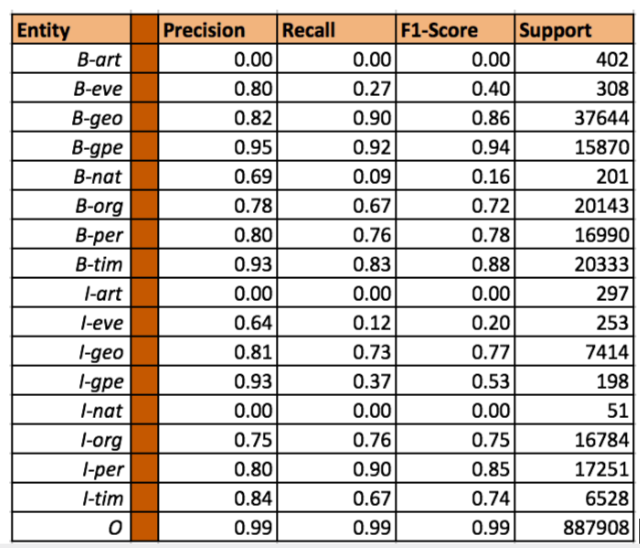
\includegraphics[h!,width=0.4\textwidth]{5folds.png}
%     \caption{5-Folds Cross Validation of NER}
%     \label{fig:5folds}
% \end{figure}

% The user study was constructed to evaluate system performance on 5 example questions, and judged by 12 respondents. Each batch of 4 respondents was additionally averaged for an average evaluation score for the system. The user study resulted in a great variety of results, and has lead us to consider many further system enhancements in an effort to alleviate some of the concerns pointed out by this user study.

% \begin{table}[h!]
% \centering
% \begin{tabular}{c}
% \hline \bf Questions Asked \\ \hline
% Who was George Washington? \\
% Name some important events in the Rev. War \\
% How was life for the Iriquois Indians?\\
% How did World War II Start? \\
% What were some reasons for the Civil War? \\
% \hline
% \end{tabular}
% \caption{\label{ques-table} Questions Asked During User Study}
% \end{table}

% In the user study, whose results can be seen in Appendix A, it can be seen that the system performs well when dealing with questions 4 and 5. However, when considering the ratings related to questions 1 and 3, the system has drastically worse performance. The results themselves are empirically obvious of the shortcomings. When looking at the related, suggested topics (as returned by the knowledge graph), a query for ‘George Washington’ returns results related to completely unrelated topics to the question such as ‘George Washington University’. This completely unrelated response is representative of a key problem with the system - the knowledge graph has no specific contextual awareness. One potential solution to this problem would be an additional layer of post processing added to the knowledge graph module. Rather than relaying the first 5 responses from the knowledge query, the system should perhaps be capable of considering the returned responses and only relating those responses considered to actually be relevant. 

% \section{Conclusion and Future Work}

% We present an alternative education solution through the use of modern information retrieval and machine learning techniques as described above. Our system can scale easily to many classes and to unlimited numbers of students By harnessing the depth and breadth of resources available online, in combination with methodology that helps establish adjacent learning with immediate feedback, proven solutions to educational problems are being implemented. While the system as it stands provides the foundation for a framework focused on this education pipeline, glaring possibilities for improvement still exist. For example, related topics as returned by our internal similarity metric are not always intuitive or useful. Future work could also explore

\bibliography{naaclhlt2018}
\bibliographystyle{acl_natbib}

\appendix

% \section{Appendix: Results from User Study}

% In Table \ref{user-table}, we see the relevance ranking of the topics returned by the knowledge graph, when supplied the questions from Table \ref{ques-table}. We then ask our users to rank the relevance of the top five returned topics, with 1 being the worst and 5 being the best. Some topics work better than others, due to the wide array of knowledge that Google's knowledge graph contains when compared to our controlled experiments. We believe that future work can help mitigate some of the low ranking responses by recommending relevant \textit{questions} from the class that the current question is also in, rather than querying an outside API.

% \begin{table}[h!]
% \begin{tabular}{|c|c|c|c|c|c|}
%     \hline \bf User & \bf Q1 & \bf Q2 & \bf Q3 & \bf Q4 & \bf Q5 \\  
%     \hline
%     \bf 1 & 1 & 3 & 2 & 4 & 4 \\ 
%     \bf 2 & 2 & 3 & 2 & 5 & 4 \\ 
%     \bf 3 & 1 & 4 & 2 & 3 & 3 \\ 
%     \bf 4 & 1 & 3 & 2 & 4 & 4 \\ 
%     \bf 5 & 2 & 5 & 2 & 5 & 4 \\ 
%     \bf 6 & 1 & 3 & 2 & 5 & 5 \\ 
%     \bf 7 & 2 & 3 & 1 & 4 & 4 \\ 
%     \bf 8 & 1 & 3 & 2 & 4 & 4 \\ 
%     \bf 9 & 1 & 4 & 3 & 5 & 4 \\ 
%     \bf 10 & 1 & 3 & 2 & 4 & 3 \\ 
%     \bf 11 & 2 & 3 & 2 & 5 & 4 \\ 
%     \bf 12 & 1 & 4 & 2 & 5 & 4 \\ 
%     \hline
%     \bf Average & \bf 1.33 & \bf 3.42 & \bf 2.00 & \bf 4.42 & \bf 3.92 \\ 
%     \hline
% \end{tabular}
% \caption{\label{user-table} Questions Asked During User Study}
% \end{table}
\end{document}